%----------------------------------------------------------------------------------------
%	PACKAGES AND OTHER DOCUMENT CONFIGURATIONS
%----------------------------------------------------------------------------------------

\documentclass[11pt, twoside]{Thesis} % The default font size and one-sided printing (no margin offsets)

\graphicspath{{Pictures/}} % Specifies the directory where pictures are stored

\usepackage{epstopdf}
\usepackage{url}
\usepackage{framed}
\usepackage[chapter]{algorithm}
\usepackage{algorithmic}
\usepackage{booktabs}
\usepackage{caption}
\usepackage{subcaption}
\usepackage{xcoffins}
\usepackage{pgffor}
\usepackage{comment}
\usepackage[toc,page]{appendix}
\usepackage[usenames,dvipsnames]{color}
\usepackage[round, comma, semicolon, sort&compress]{natbib} % Use the natbib reference package - read up on this to edit the reference style; if you want text (e.g. Smith et al., 2012) for the in-text references (instead of numbers), remove 'numbers' 
%\usepackage{todonotes}
\usepackage{pdfpages}

\hypersetup{
urlcolor=black,
colorlinks=true,
linkcolor=MidnightBlue,
citecolor=BrickRed,
linktocpage
} % Colors hyperlinks in blue - change to black if annoying
\title{\ttitle} % Defines the thesis title - don't touch this

\begin{document}
\frontmatter % Use roman page numbering style (i, ii, iii, iv...) for the pre-content pages

\setstretch{1.3} % Line spacing of 1.3

% Define the page headers using the FancyHdr package and set up for one-sided printing
\fancyhead{} % Clears all page headers and footers
\rhead{\thepage} % Sets the right side header to show the page number
\lhead{} % Clears the left side page header

\pagestyle{fancy} % Finally, use the "fancy" page style to implement the FancyHdr headers

\newcommand{\HRule}{\rule{\linewidth}{0.5mm}} % New command to make the lines in the title page


\newcommand{\todo}[1]{{\color{red}\fbox{\color{blue}#1}}}



\NewCoffin\tablecoffin
\NewDocumentCommand\Vcentre{m}
  {%
    \SetHorizontalCoffin\tablecoffin{#1}%
    \TypesetCoffin\tablecoffin[l,vc]%
  }

% PDF meta-data
\hypersetup{pdftitle={\ttitle}}
\hypersetup{pdfsubject=\subjectname}
\hypersetup{pdfauthor=\authornames}
\hypersetup{pdfkeywords=\keywordnames}

\includepdf[offset=2.55cm -2.55cm]{cover.pdf}
%----------------------------------------------------------------------------------------
%	TITLE PAGE
%----------------------------------------------------------------------------------------

\cleardoublepage
\pagestyle{empty}
\null\vfill
{\Large
The present work has been conducted in association with the \emph{Advanced Concepts Team} (ACT) in \emph{European Space Agency} (ESA-ESTEC, Noordwijk) and the University of Amsterdam. The subject of this work had been offered as an internship project by the ACT under the title: ``\textit{Simultaneous evolution of morphology and locomotion of soft robots by novelty search}''. Most of this work has been conducted during my $3$-month internship at the ACT, ESA-ESTEC. The resulted work was also submitted in partial fulfillment of the requirements for the degree of MSc. Artificial Intelligence of the University of Amsterdam as a master thesis.}
\vfill\null


\begin{titlepage}

\begin{center}
\includegraphics[width=.10\textwidth]{../Figures/Misc/University_of_Amsterdam_logo.pdf}\\[0.2cm]
\textsc{\Large \univname}\\[0.7cm] % University name
\textsc{\LARGE Master Artificial Intelligence}\\[2.0cm]
\vspace{0.1cm}% University/department logo - uncomment to place it
\textsc{\large Master Thesis}\\[0.5cm]
\HRule \\[0.4cm] % Horizontal line
{\huge \bfseries \ttitle}\\[0.4cm] % Thesis title
\HRule \\[1.5cm] % Horizontal line
\begin{minipage}[t][3.5cm][t]{0,4\textwidth}
\begin{flushleft} \large
\emph{Author:}\\
\authornames
\end{flushleft}
\end{minipage}
\begin{minipage}[t][3.5cm][t]{0,4\textwidth}
\begin{flushright} \large
\emph{Supervisors:} \\
\supname
\end{flushright}
\end{minipage}
\begin{flushbottom}
\begin{center}
ECTS: $42$\\[0.5cm]
\textit{Submitted to the Board of Examiners in partial\\ fulfillment of the requirements for the degree of \\\textbf{MSc. Artificial Intelligence}\\ of the\\ \textsc{University of Amsterdam}.}\\[2.5cm]
\large \today
\end{center}
\end{flushbottom}
\end{center}
\end{titlepage}

\cleardoublepage



%----------------------------------------------------------------------------------------
%	DECLARATION PAGE
%	Your institution may give you a different text to place here
%----------------------------------------------------------------------------------------

\clearpage % Start a new page

%----------------------------------------------------------------------------------------
%	QUOTATION PAGE
%----------------------------------------------------------------------------------------

\pagestyle{empty} % No headers or footers for the following pages

\null\vfill % Add some space to move the quote down the page a bit

\textit{``Evolve solutions; when you find a good one, don't stop."}

\begin{flushright}
David Eagleman, \textit{Incognito: The Secret Lives of the Brain}
\end{flushright}

\vfill\vfill\vfill\vfill\vfill\vfill\null % Add some space at the bottom to position the quote just right

\cleardoublepage % Start a new page

%----------------------------------------------------------------------------------------
%	ABSTRACT PAGE
%----------------------------------------------------------------------------------------

\addtotoc{Abstract} % Add the "Abstract" page entry to the Contents

\abstract{\addtocontents{toc}{\vspace{1em}} % Add a gap in the Contents, for aesthetics
Soft robotics is a vivid research field on the science and engineering aspects of soft materials in mobile machines. Recent development in soft robotics and evolutionary optimization have shown the ability to simultaneously evolve the morphology and locomotion of soft robots. Generative encoding coupled with neural evolution of augmented topologies shows promising results. Novelty search, unlike traditional optimization methods does not aim to optimize the objective but instead looks for novelty. Novelty search rewards diversity and leads to a  variety of solutions, mimicking natural evolution. Apart from the performance comparison between novelty and fitness based search, this thesis shows that new locomotion patterns can be produced by the former. Different types of selection algorithms for fitness and novelty based evolution are studied. In addition, a method to combine both is proposed. Finally, the performance objective-wise is tested under variant gravity conditions leading into a taxonomy of possible locomotion strategies given different gravity levels.
}

\clearpage % Start a new page

%----------------------------------------------------------------------------------------
%	ACKNOWLEDGEMENTS
%----------------------------------------------------------------------------------------

\setstretch{1.3} % Reset the line-spacing to 1.3 for body text (if it has changed)

\acknowledgements{\addtocontents{toc}{\vspace{1em}} % Add a gap in the Contents, for aesthetics
The present work has been conducted in association with the \emph{Advanced Concepts Team} (ACT) in \emph{European Space Agency} (ESA-ESTEC, Noordwijk). The subject of this thesis had been offered as an internship project by the ACT under the title: ``\textit{Simultaneous evolution of morphology and locomotion of soft robots by novelty search}''. Most of this work has been conducted during my $3$-month internship at the ACT, ESA-ESTEC.

It would have been impossible to write this thesis without the help and support of my three supervisors, Arnoud Visser (Senior Lecturer, UvA), Dario Izzo (Scientific Coordinator, ACT) and Daniel Hennes (Postdoctoral Research Fellow, ACT).

I would like to thank Arnoud for his valuable comments in the whole duration of this thesis. I am grateful for all the discussion we had the last two years regarding my thesis, Dutch Nao Team, and the number of projects and papers we have done together.

I am most grateful to Dario and Daniel. Their ideas and discussions we had were valuable for me to finish this work. It has been an honor working under their supervision, as I gained too much from them.

I express my warm thanks to all the members of Dutch Nao Team, the Robocup SPL team of University of Amsterdam, in which I was proud to serve as a member for two years. I also thank all the members of ACT who welcomed me in the team and made my three-month internship a wonderful experience. Special thanks to Paul for our ``evolutionary'' conversations.

I would like to express my gratitude towards everyone who supported me during my master studies. Especially, my family, my friends, and my girlfriend. You have given me your unequivocal support throughout this work and my studies.
}
\clearpage % Start a new page

%----------------------------------------------------------------------------------------
%	LIST OF CONTENTS/FIGURES/TABLES PAGES
%----------------------------------------------------------------------------------------

\pagestyle{fancy} % The page style headers have been "empty" all this time, now use the "fancy" headers as defined before to bring them back

\newpage
\lhead{\emph{Contents}} % Set the left side page header to "Contents"
\tableofcontents % Write out the Table of Contents

\newpage
\lhead{\emph{List of Figures}} % Set the left side page header to "List of Figures"
\listoffigures % Write out the List of Figures

\newpage
\lhead{\emph{List of Tables}} % Set the left side page header to "List of Tables"
\listoftables % Write out the List of Tables

\newpage
\lhead{\emph{List of Algorithms}} % Set the left side page header to "List of Tables"
{\let\clearpage\relax\listofalgorithms}
\addcontentsline{toc}{chapter}{List of algorithms}

\clearpage % Start a new page

%----------------------------------------------------------------------------------------
%	ABBREVIATIONS
%----------------------------------------------------------------------------------------

%\clearpage % Start a new page
%
%\setstretch{1.5} % Set the line spacing to 1.5, this makes the following tables easier to read
%
%\lhead{\emph{Abbreviations}} % Set the left side page header to "Abbreviations"
%\listofsymbols{ll} % Include a list of Abbreviations (a table of two columns)
%{
%\textbf{LAH} & \textbf{L}ist \textbf{A}bbreviations \textbf{H}ere \\
%%\textbf{Acronym} & \textbf{W}hat (it) \textbf{S}tands \textbf{F}or \\
%}

%----------------------------------------------------------------------------------------
%	PHYSICAL CONSTANTS/OTHER DEFINITIONS
%----------------------------------------------------------------------------------------

%\clearpage % Start a new page
%
%\lhead{\emph{Physical Constants}} % Set the left side page header to "Physical Constants"
%
%\listofconstants{lrcl} % Include a list of Physical Constants (a four column table)
%{
%Speed of Light & $c$ & $=$ & $2.997\ 924\ 58\times10^{8}\ \mbox{ms}^{-\mbox{s}}$ (exact)\\
%% Constant Name & Symbol & = & Constant Value (with units) \\
%}

%----------------------------------------------------------------------------------------
%	SYMBOLS
%----------------------------------------------------------------------------------------

%\clearpage % Start a new page
%
%\lhead{\emph{Symbols}} % Set the left side page header to "Symbols"
%
%\listofnomenclature{lll} % Include a list of Symbols (a three column table)
%{
%$a$ & distance & m \\
%$P$ & power & W (Js$^{-1}$) \\
%% Symbol & Name & Unit \\
%
%& & \\ % Gap to separate the Roman symbols from the Greek
%
%$\omega$ & angular frequency & rads$^{-1}$ \\
%% Symbol & Name & Unit \\
%}

%----------------------------------------------------------------------------------------
%	DEDICATION
%----------------------------------------------------------------------------------------
\clearpage

\setstretch{1.3} % Return the line spacing back to 1.3

\pagestyle{empty} % Page style needs to be empty for this page

\dedicatory{This work is dedicated to my family. Thank you for your support during all the years I have been a student.} % Dedication text

\addtocontents{toc}{\vspace{2em}} % Add a gap in the Contents, for aesthetics

%----------------------------------------------------------------------------------------
%	THESIS CONTENT - CHAPTERS
%----------------------------------------------------------------------------------------

\mainmatter % Begin numeric (1,2,3...) page numbering

\pagestyle{fancy} % Return the page headers back to the "fancy" style

% Include the chapters of the thesis as separate files from the Chapters folder
% Uncomment the lines as you write the chapters

% Chapter 1

\chapter{Introduction} % Main chapter title

\label{Chapter1} % For referencing the chapter elsewhere, use \ref{Chapter1} 

\lhead{Chapter 1. \emph{Introduction}} % This is for the header on each page - perhaps a shortened title


Soft robotics is a field of research inspired by soft-bodied organisms, whereas the engineering and designing aspects of soft-structures are in the middle of interest, as soft-robotics can make the interaction between robots and living organisms safe, as well as their function in natural or more complex environments, where rigid robots have disadvantages. Actuated soft materials that react to environmental changes, add complexity to the designing phase of soft-robot engineering, since the degrees of freedom for soft structures that the distribution of materials and the space of possible morphologies, make the number of possibilities vast. 

Approaching such vast search spaces, is a heavy task, recent development in evolutionary optimization though, have shown the possibility of successful evolution of both the morphology and the locomotion strategy of soft robots, while the genotype representation is of vital importance to the evolution. Generative encoding for the genotype representation has shown promising results. Compared to direct encoding, where its representation is a direct mapping from genotype to phenotype level, generative encoding genotype is a function that is similar to a set of rules that can be queried for each coordinate in the Cartesian phenotype space and produce the output. Recent work has proved that evolutionary methods coupled with a generative encoding genotype representation can actually evolve both the morphology and the locomotion behavior of soft-robotics in a virtual simulation.

Traditional evolutionary methods in pursuance of the objective function defined by the user, are blind to keep enough diversity within the population, resulting usually driving the evolution towards local optima. Novelty search, unlike traditional optimization methods does not aim to optimize individuals towards an objective, but instead looks for novelty. Novelty search rewards diversity and leads to a boundless variety of solutions, mimicking natural evolution in such a way. Doing so, it has proven to be a successful method for searching vast spaces where the objective function is deceptive.

Passive soft-robotic structures have no limitations to the extent of morphologies, in the same context, gravity conditions when robot locomotion is investigated might be more decisive when it comes to the morphology of the robot explorers. With the freedom soft-structures can give to evolutionary techniques in respect to the designing part of the evolution (evolved morphology), it is of interest to validate that a taxonomy of different locomotion strategies can apply when the gravity conditions change.



\section{Thesis Contribution}

This thesis explores possibles ways of evolving the morphology and the locomotion strategy of soft structures under a virtual simulation environment. A simple genetic algorithm is used to confirm that these kind of problems cannot be captured by a simple genetic method, with direct encoding representation. Direct and direct encoding are also used under a random robot generator which show the advantages of the encoding in the produced structures, as well as point out the need of an indirect encoding to explore and exploit the geometrical properties of the problem. This encoding scheme is used paired to an evolutionary algorithm to verify results of previous work on the same domain, showing that generative representations for the genotype can indeed benefit these kind of evolutionary optimization methods. In addition, this thesis is exploring the effect of diversity based evolution can have in the performance of the evolved morphologies. Novelty search, a method rewarding the ``new'' in the behavior level is used for this purpose showing that not only same or better performance can be achieved through this method but also the diversity of behaviors is remarkably increased. \todo{write for different gravities...}






\section{Thesis Outline}

Chapter~\ref{Background}, provides some background information on the field of soft robotics, an introduction to genetic algorithms, different encoding techniques for the genomes, neuroevolution algorithms, and finally, objective driven search is presented and compared to novelty search. In Chapter~\ref{Related Work}, related material about evolutionary techniques for evolution of soft-robots morphology and locomotion is presented, in aspects of artificial life. Chapter~\ref{Method}, is a comprehensive documentation presenting details of the implementation of different evolutionary techniques. Chapter~\ref{Results}, gives a detailed presentation of the results achieved under variant techniques. Next, in chapter~\ref{Future Work}, future applications and extensions of this work provided. Chapter~\ref{Conclusion}, serves as an epilogue to this thesis, where some important points of it are presented.
% Chapter 2

\chapter{Related Work} % Main chapter title

\label{Chapter2} % For referencing the chapter elsewhere, use \ref{Chapter1} 

\lhead{Chapter 2. \emph{Related Work}} % This is for the header on each page - perhaps a shortened title
% Chapter 3

\chapter{Results} % Main chapter title

\label{Results} % For referencing the chapter elsewhere, use \ref{Chapter1} 

\lhead{Chapter 3. \emph{Results}} % This is for the header on each page - perhaps a shortened title

\section{Results}

\clearpage
\subsection{Fitness Based Search}

\begin{figure}[h!]
\centering
\includegraphics[width=1.0\textwidth]{../Figures/Results/indRunsSize10Fitness.pdf}
\caption{Caption}
\caption{Best so far fitness in body lengths displacement of softbot's center of mass from $10$ runs for fitness based search. The gravity acceleration for this experiment used was $-27.468\   m/s^2$, the size of the lattice $10\times 10\times10$ and $4$ available materials ($2$-actuated).}
\end{figure}

\begin{figure}[h!]
\centering
\includegraphics[width=1.0\textwidth]{../Figures/Results/indRunsAvgSize10Fitness.pdf}
\caption{Best so far fitness in body lengths displacement of softbot's center of mass from $10$ runs together with their mean (thick line) for fitness based search. The gravity acceleration for this experiment used was $-27.468\   m/s^2$, the size of the lattice $10\times 10\times10$ and $4$ available materials ($2$-actuated).}
\label{fig:indRunsAvgSize10Fitness}
\end{figure}

\clearpage
\subsection{Novelty Search}

\begin{figure}[h!]
\centering
\includegraphics[width=1.0\textwidth]{../Figures/Results/indRunsSize10Novelty.pdf}
\caption{Best so far fitness in body lengths displacement of softbot's center of mass from $10$ runs for novelty search. The gravity acceleration for this experiment used was $-27.468\   m/s^2$, the size of the lattice $10\times 10\times10$ and $4$ available materials ($2$-actuated).}
\label{fig:indRunsSize10Novelty}
\end{figure}

\begin{figure}[h!]
\centering
\includegraphics[width=1.0\textwidth]{../Figures/Results/indRunnAvgSize10Novelty.pdf}
\caption{Best so far fitness in body lengths displacement of softbot's center of mass from $10$ runs together with their mean (thick line) for novelty search. The gravity acceleration for this experiment used was $-27.468\   m/s^2$, the size of the lattice $10\times 10\times10$ and $4$ available materials ($2$-actuated).}
\label{fig:indRunnAvgSize10Novelty}
\end{figure}


\begin{figure}
\centering
\includegraphics[width=1.0\textwidth]{../Figures/Results/KnnExperimentSize5.pdf}
\caption{Novelty search - best so far fitness in body lengths displacement of softbot's center of mass from $10$ runs together with their mean (thick line). The novelty is computed as the average distance from the $K$-nearest behaviors for $K \in \lbrace 1,2,5,10,20 \rbrace $. The gravity acceleration for this experiment used was $-27.468\   m/s^2$, the size of the lattice $5\times 5\times5$ and $4$ available materials ($2$-actuated).}
\label{fig:KnnExperimentSize5}
\end{figure}


\clearpage
\subsection{Novelty-Fitness Based Search Comparison}

\begin{figure}[h!]
\centering
\includegraphics[width=1.0\textwidth]{../Figures/Results/FitvsNovVsDirSize5.pdf}
\caption{Best so far fitness in body lengths displacement of softbot's center of mass averaged over $10$ runs together with the standard deviation error. The gravity acceleration for this experiment used was $-27.468\   m/s^2$, the size of the lattice $5\times 5\times5$ and $4$ available materials ($2$-actuated).}
\label{fig:FitvsNovVsDirSize5}
\end{figure}

\begin{figure}[h!]
\centering
\includegraphics[width=1.0\textwidth]{../Figures/Results/AvgGenerChampNoveltyFitnessSize5.pdf}
\caption{Fitness of the generation champion (best individual) per generation in body lengths displacement of softbot's center of mass averaged over $10$ runs together with the standard deviation error. The gravity acceleration for this experiment used was $-27.468\   m/s^2$, the size of the lattice $5\times 5\times5$ and $4$ available materials ($2$-actuated).}
\label{fig:AvgGenerChampNoveltyFitnessSize5}
\end{figure}

\begin{figure}[h!]
\centering
\includegraphics[width=1.0\textwidth]{../Figures/Results/FitvsNovVsDirSize10.pdf}
\caption{Best so far fitness in body lengths displacement of softbot's center of mass averaged over $10$ runs together with the standard deviation error. The gravity acceleration for this experiment used was $-27.468\   m/s^2$, the size of the lattice $10\times 10\times10$ and $4$ available materials ($2$-actuated).}
\label{fig:FitvsNovVsDirSize10}
\end{figure}

\begin{figure}
\centering
\includegraphics[width=1.0\textwidth]{../Figures/Results/ViolinPlotsAvgGenFitSize5.pdf}
\caption{Distributions of average population fitness per generation over 10 runs. The gravity acceleration for this experiment used was $-27.468\   m/s^2$, the size of the lattice $5\times 5\times5$ and $4$ available materials ($2$-actuated). Blue (Novelty search), Green(Fitness based search).}
\label{fig:ViolinPlotsAvgGenFitSize5}
\end{figure}


\begin{figure}
\centering
\includegraphics[width=1.0\textwidth]{../Figures/Results/novelIndividualsFitNovComp.pdf}
\caption{Novel individual's behaviors upto generation averaged over 10 runs. The novelty is computed as the average distance from the $10$-nearest behaviors. The gravity acceleration for this experiment used was $-27.468\   m/s^2$, the size of the lattice $5\times 5\times5$ and $4$ available materials ($2$-actuated). Blue (Novelty search), Green (Fitness based search).}
\label{fig:ViolinPlotsAvgGenFitSize5}
\end{figure}



\begin{figure}
\centering
\includegraphics[width=1.0\textwidth]{../Figures/Results/FitNovRandomDirectSize5.pdf}
\caption{Best so far fitness in body lengths displacement of softbot's center of mass averaged over $10$ runs together with the standard deviation error. The gravity acceleration for this experiment used was $-27.468\   m/s^2$, the size of the lattice $5\times 5\times5$ and $4$ available materials ($2$-actuated).}
\label{fig:FitNovRandomDirectSize5}
\end{figure}

\begin{figure}
\centering
\includegraphics[width=1.0\textwidth]{../Figures/Results/FitNovRandomSize5.pdf}
\caption{Best so far fitness in body lengths displacement of softbot's center of mass averaged over $10$ runs together with the standard deviation error. The gravity acceleration for this experiment used was $-27.468\   m/s^2$, the size of the lattice $5\times 5\times5$ and $4$ available materials ($2$-actuated).}
\label{fig:FitNovRandomSize5}
\end{figure}


\begin{figure}
\centering
\includegraphics[width=1.0\textwidth]{../Figures/Results/FitNovSize5Pen2.pdf}
\caption[]{Best so far fitness averaged over $10$ runs together with the standard deviation error penalizing actuated materials\footnotemark. The gravity acceleration for this experiment used was $-27.468\   m/s^2$, the size of the lattice $5\times 5\times5$ and $4$ available materials ($2$-actuated).}
\label{fig:FitNovRandomSize5}
\end{figure}

\footnotetext{Actuated materials penalize fitness: \[f = (1 - (n_{actuated} / n_{total})^{1.5}) \times disp \], where $n_{actuated}$, is the number of actuated voxels, $n_{total}$ total number of voxels and $disp$ the displacement of the softbot's center of mass.}

\clearpage
\subsection{Local competition in fitness based evolution}

\begin{figure}[h!]
\centering
\includegraphics[width=1.0\textwidth]{../Figures/Results/fitComp100_20percent.pdf}
\caption{Best so far fitness in body lengths displacement of softbot's center of mass averaged over $10$ runs together with the standard deviation error. Local competition is held among the top $20\%$ and in the complete population of each species. The gravity acceleration for this experiment used was $-27.468\   m/s^2$, the size of the lattice $5\times 5\times5$ and $4$ available materials ($2$-actuated).}
\label{fig:fitComp100_20percent}
\end{figure}

\begin{figure}[h!]
\centering
\includegraphics[width=1.0\textwidth]{../Figures/Results/FitVsFitCompSize5.pdf}
\caption{Best so far fitness in body lengths displacement of softbot's center of mass averaged over $10$ runs together with the standard deviation error. Local competition is held among the top $20\%$ of each species population. The gravity acceleration for this experiment used was $-27.468\   m/s^2$, the size of the lattice $5\times 5\times5$ and $4$ available materials ($2$-actuated).}
\label{fig:FitVsFitCompSize5}
\end{figure}

\begin{figure}[h!]
\centering
\includegraphics[width=1.0\textwidth]{../Figures/Results/fitComp100percent.pdf}
\caption{Best so far fitness in body lengths displacement of softbot's center of mass averaged over $10$ runs together with the standard deviation error. Local competition is held among the complete population of each species. The gravity acceleration for this experiment used was $-27.468\   m/s^2$, the size of the lattice $5\times 5\times5$ and $4$ available materials ($2$-actuated).}
\label{fig:fitComp100percent}
\end{figure}


\clearpage
\subsection{Local competition in novelty search evolution}

\begin{figure}[h!]
{\centering
\includegraphics[width=1.0\textwidth]{../Figures/Results/NoveltyCompetitionsSize5.pdf}}
\caption{Best so far fitness in body lengths displacement of softbot's center of mass averaged over $10$ runs together with the standard deviation error. Local competition is held among the complete population of each species. The gravity acceleration for this experiment used was $-27.468\   m/s^2$, the size of the lattice $5\times 5\times5$ and $4$ available materials ($2$-actuated).}
\label{fig:NoveltyCompetitionsSize5}
\end{figure}
% Chapter 4

\chapter{Method} % Main chapter title

\label{Method} % For referencing the chapter elsewhere, use \ref{Chapter1} 

\lhead{Chapter 4. \emph{Method}} % This is for the header on each page - perhaps a shortened title


In this chapter, an introduction to the problem specifications and a comprehensive documentation describing the methods used is given. As an initial experiment, a random methodology has been implemented to verify that random non-evolutionary approaches fail in such settings. Next, evolutionary methods are used in order the morphology and the locomotion strategy of soft-robots to be co-evolved in the simulated environment. A direct encoding genetic algorithm is used as in~\citep{cheney2013unshackling}. This direct encoding is expected to be unable to evolve efficient locomotion due to the irregular morphologies direct encoding is expected to produce. Furthermore, a generative encoding, named CPPN, is used and paired with NEAT evolutionary algorithm in order a baseline for the following experiments will be created, verifying previous work~\citep{cheney2013unshackling}.

Novelty search is the main methodology investigated in this thesis. The implementation of this method alters the pipeline of the NEAT evolutionary algorithm to fit the new objective function. Pure novelty search used to evolve three dimensional virtual creatures in a simulated environment~\citep{lehman2011evolving}, using a behavior metric such as the morphology of the produced creature, failed to compete with the traditional fitness-based search. In addition to the discussion regarding the above method, behavior metrics can be used in this problem domain are investigated. 



\section{Problem Introduction}

Recent work in evolutionary robotics shows that compositional pattern producing networks (CPPNs) can encode soft-robot morphologies. These networks can produce regular outputs which is translated to regular shapes for the structures produced, resulting in efficient movement. VoxCad simulator provides a test-bench for analyzing soft-robot bodies that can be actuated through environmental changes, in the specific case the temperature. In addition to that, recent work by~\citep{cheney2013unshackling}, showed that very interesting morphologies can be evolved by the CPPN-NEAT algorithm in the specific soft-robot simulation environment.

\paragraph*{VoxCad}~\\

For the simulation of the soft material bodies, VoxCad's~\citep{hiller2012dynamic} underlying physics engine \emph{Voxelyze} was used as a stand-alone software to analyze the soft structures without the computational cost of rendering. As far as the soft-material simulation settings are concerned, it is not of interest for this thesis to explore the best not only environmental but also material settings for the evolved soft-robots. All variables of the environment, excluding the temperature period and the gravity acceleration, are constants throughout this thesis. Table~\ref{VoxelyzeSimulationSettings}, describes and presents the values used in different variables of the simulation.



\paragraph*{Materials}~\\

\begin{figure}
\centering
\includegraphics[height=0.2\textheight]{../Figures/Misc/allSoftMaterials.png}
\caption{Soft robot uses four materials (two active, two passive), morphology evolved penalizing actuated materials.}
\label{fig:allSoftMaterials}
\end{figure}

Within the VoxCad simulation software there is the option of defining and using a palette of materials. Materials can be \emph{passive} or \emph{active}. Passive materials do not react to temperature changes while active materials expand and contract in respect to their thermal properties. Figure~\ref{fig:allSoftMaterials}, illustrates a soft robot consisting of all four materials used in the experiments. \textcolor{Red}{Red} and \textcolor{Green}{Green} are the only actuated materials with non-zero and opposite thermal expansion coefficients, meaning that their phase in respect to the actuation from temperature changes is equal to half a circle, green voxels contract the same time red expand and vice versa, mimicking living organisms' muscle tissue. The two additional materials represent soft non-actuated tissue that can be soft (soft tissue) or hard (bones). \textcolor{Cyan}{Cyan} voxels are soft, having five times smaller elastic modulus of their material than \textcolor{Blue}{Blue} which have $50$ \texttt{MPa}.


\section{Random Generation of Soft-Robots}

To evaluate all the following evolutionary methods used, information about the performance of random generated morphologies must be present. In order to achieve that, two random approaches which will also help the understanding between direct and indirect encoding implemented. 

The first implementation of a random morphology generator mimics ``direct'' encoding. This method assigns randomly the presence of a voxel in the three dimensional space of the lattice. The probability of adding a voxel in given coordinates is $0.5$. The material of each presented voxel is chosen a random material from the palette. Each material has the same propability of being chosen. After all voxels have been assigned a material, unconnected parts of of the structure will be removed, keeping only the largest connected structure in the lattice.


\begin{figure}
\centering
\includegraphics[width=1.0\textwidth]{../Figures/Results/random.pdf}\\
\hspace{0.1cm}
\includegraphics[height=0.15\textwidth]{../Figures/Robots/random.jpg}
\includegraphics[height=0.15\textwidth]{../Figures/Robots/rg0.jpg}
\includegraphics[height=0.15\textwidth]{../Figures/Robots/rg1.jpg}
\caption{Generative encoding creates more natural morphologies even in random schemes (see Settings~\ref{Settings-size10}).}
\label{fig:randomResultsRobots}
\end{figure}

An ``indirect'' way of producing random morphologies, follows a different method of assigning materials to voxels, following a set of rule in order a new morphology to be produced. This method holds two probabilities, the one refers to the probability of adding a new voxel in the already generated structure, the next one denotes the probability that the material of a new inserted voxel will be the same as the one of the material is going to be connected to. First, a random material voxel is inserted in a random coordinate into the lattice. When a new voxel is to be added, a connection (voxel) is chosen from the already inserted voxels. The side of the connection is chosen from a uniform distribution out of all valid (within the lattice space) sides. In this generative process there is also the possibility of creating structures in half of the lattice space, and then mirror the soft structures in both halves of it, generating symmetrical morphologies.

Considering these three methods, the difference between direct and indirect coding, presented in section~\ref{DirectIndirect}, is becoming easier interpreted. In the ``direct'' process, a probability determines the presence and the material of every voxel in the lattice. On the other hand, in the ``generative'' method a set of rules and probabilities define the structure that is going to be produced into the available space.

Figure~\ref{fig:randomResultsRobots}, illustrates not only the actual performance (fitness in body lengths traveled by top-$1000$ soft-robots from $30000$ total runs for each method) of the previously described methods, but also one of the best performing soft-robots of each method. Both ``generative'' methods outperform the ``direct'' one, mostly because they are capable of generating regular morphologies. ``Generative'' random soft-robot generation methods create more compact structures which can move easier due to their size and their geometrical features. For the \textit{Generative-Mirrored} approach even though the average performance is slightly worse than the plain method it actually performs way better in some distinct cases (outliers). Adding geometrical properties resulted in getting more efficient locomotion by the generated soft-robots.

All methods achieved an average displacement of the soft-robots around or more than one body length, which is considered to be very low in respect to the robots generated by evolutionary methods will be presented later in this thesis.

\section{Direct-Encoded Evolutionary Soft-Robots}
\label{DirectEncodingEvolution}

\begin{figure}
\centering
\includegraphics[height=0.2\textheight]{../Figures/Robots/direct.jpg}
\caption{Direct encoding cannot capture the geometrical properties of some problems.}
\label{fig:directRobot}
\end{figure}

In the previous section, three random methodologies of ``indirect'' and ``direct'' generation of soft-robots implemented, failing to produce any decent locomotion gaits for the soft structures. Considering how vast is the solution space, random approaches are doomed to fail in a definite number of tries. Therefore, a more sophisticated evolutionary method is discussed here.

Direct encoding genomes coupled with a simple genetic algorithm is a successful approach in evolving robot controllers. As it was previously stated in ch.~\ref{Background}, mutations and crossovers of real value streams, search the problem space effectively finding near optimal solutions in demanding optimization problem domains. The GAlib C++ library \citep{wall1996galib} is used for the implementation of this method.

\paragraph*{Representation of the genotype}~\\
As in every direct encoding scheme, genotype can be represented by a stream of bits, which length is equal to the number of the dimensions of the problem. The capacity of the materials' palette is the first dimensions of the problem. The presence or not of a material at a given position in the lattice space adds one more dimension to the representation. Analytically, its length can be represented by a stream of length equal to the number of voxels in the lattice times the materials used plus one denoting the presence of a material, described by the following equation:
\begin{equation}
\label{lengthDirect}
| Genome | = (l_x \times l_y \times l_z ) \times (1 + |p|)
\end{equation}
, where $l_x, l_y, l_z$ are the dimensions of the lattice space, and $p$ is the palette of materials.
\begin{equation*}
Genome = \underbrace{01010\ldots011011}_\text{Presence}\ \    \underbrace{10101\ldots110011}_{Material_1} \   \ldots\  \underbrace{00011\ldots111110}_{Material_n}
\end{equation*}
The above stream of bit illustrates how a soft-structure in VoxCad environment can be represented by a direct encoding scheme. Each of the values of the stream is represented by a float value between zero and one, which in lower-level is represented by a stream of bits. The mapping from the genotype level to the phenotype is straightforward in this case, the first stream of values is used to determine the presence or not for a voxel, while in case of a presence the other $n$ streams are used and the maximum value in specific positions of the streams determine the material is going to be used.

Considering the representation of the genome, as well as the geometrical nature of the problem it self, it is valid to say that we do not expect that direct encoding will capture this major property of the problem (see Fig.~\ref{fig:directRobot}). Thus, it is not expected this stream of bits being able to generate soft-robots that can locomote efficiently.





\section{Generative-Encoded Evolutionary Soft-Robots}

Direct encoding methods lack the morphology regularities of the evolved soft-robots. Compositional pattern-producing networks (CPPNs), can serve this function. Compositional pattern producing networks are built up by a set of canonical functions which force the outputs of the network to produce repetitive, symmetrical and geometrically interesting patterns. Producing regularities in the phenotype space, and capturing geometrical properties of the optimization problem, it is expected to produce efficient locomotion strategies and morphologies of the soft structures~\citep{cheney2013unshackling}.
\begin{figure}
\centering
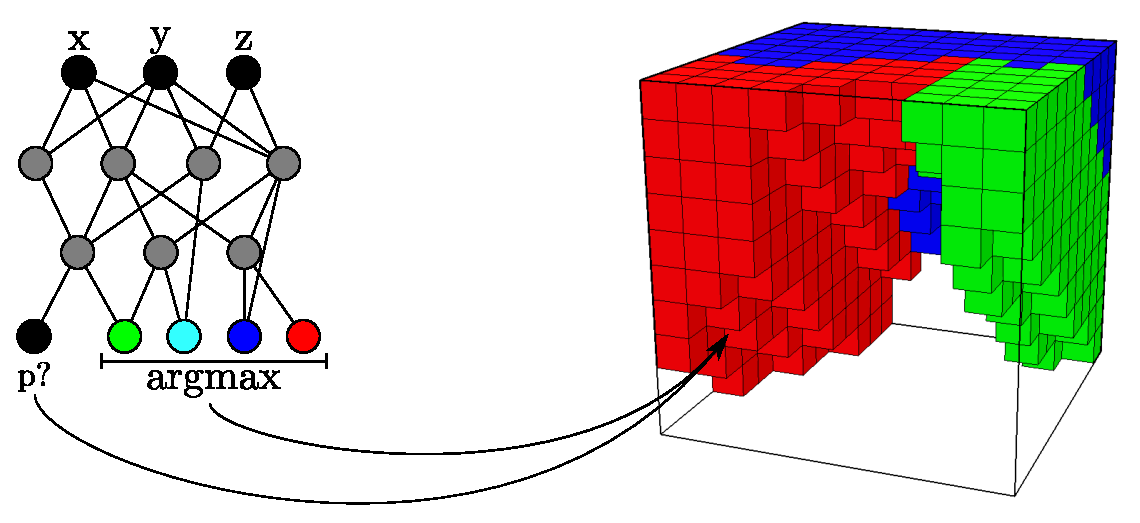
\includegraphics[height=0.2\textheight]{../Figures/Misc/cppnSoftBot.eps}
\caption{Each genotype is queried for every coordinate inside the lattice, its outputs determine the presence of a voxel and the type of its material.}
\label{fig:cppnDiagram}
\end{figure}
Since, CPPNs must be queried for every coordinate of the lattice space, the input nodes (neurons) of the CPPN are assigned to x,y,z normalized coordinates following~\citep{cheney2013unshackling} so that:
\[x,y,z \in [-1,1]\]
A bias input node is also introduced in the genome CPPN representation. More inputs could be added to the CPPNs, for instance the distance from the center point of the Cartesian space (simulation lattice) as described in~\citep{stanley2007compositional} and used in~\citep{cheney2013unshackling}, which naturally adds more bias towards symmetrical structures. However, evolving perfectly symmetrical structures is not much of an interest to show, since CPPNs, as it is shown later in this thesis, can evolve symmetrical morphologies without this extra information input node(s). The proposed input nodes for the three dimensions of the Cartesian space provide the minimum bias to the network outputs. Figure~\ref{fig:cppnDiagram}, illustrates the topology of a random CPPN network with the input and output nodes described above. The set of nodes and connections determine the network's \emph{topology}. The topology of these networks can be variant and be evolved alongside the weights of the connections in any neuroevolutionary method. The divergent part of the network between the input and the output nodes is described by the genotype and it is the one that is going to be evolved and altered during the evolution. The presence or not of a voxel in each coordinate of the lattice is determined by a single output of the CPPN called $p$ and the selection of the material is determined by $n$-outputs. The node with the maximum value in the output will determine which of the materials will be used.

\subsection{How CPPNs can be evolved?}

The evolution of these indirect representations of the phenotypes can be evolved with any method able to evolve artificial neural networks, since they are identical with CPPNs. CPPN-NEAT (see Section~\ref{CPPN}), is a method of evolving CPPNs within NEAT evolutionary method. Previous work~\citep{cheney2013unshackling}, showed that this method can indeed evolve the morphologies of the soft-robots in the VoxCad simulation environment. HyperNEAT\footnote{HyperNEAT \texttt{v4.0 C++} by J. Gauci code (url: \url{https://github.com/MisterTea/HyperNEAT})} was used for the implementation of the CPPN-NEAT algorithm. Algorithm~\ref{evolutionPseudocode}, presents the pseudocode for the evolution under CPPN-NEAT method. In addition, a brief explanation of each function used in the algorithm follows:


\begin{algorithm}[t!]
\caption{CPPN-NEAT evolution}
\label{evolutionPseudocode}
\begin{algorithmic}[1]
\STATE $\mathtt{population} = \varnothing$
\STATE $\mathtt{species} = \varnothing$
\STATE $\mathtt{generation}[0] = \mathbf{initial\_population}()$
\FOR{ $i = 0\   \text{to}\  \mathtt{max\_generation}$}
\STATE $\mathtt{species} = \mathtt{species} \cup \mathbf{speciation}(\mathtt{generation}[i])$
\STATE $\mathbf{evaluation}(\mathtt{generation}[i])$
\STATE $\mathbf{adjust\_fitness}(\mathtt{generation}[i], \mathtt{species})$
\STATE $\mathbf{selection}(\mathtt{generation}[i], \mathtt{species})$
\STATE $\mathtt{generation}[i+1] = \mathbf{reproduction}(\mathtt{generation}[i])$
\STATE $\mathtt{population} = \mathtt{population} \cup \mathtt{generation}[i+1]$
\ENDFOR
\end{algorithmic}
\end{algorithm}

\begin{description}
\item[Initial population]{Before the evolution starts, an initial population must be produced, identical genomes (CPPNs), with variant connection weights fill up the population.}

\item[Speciation]{Takes place and split the population in separate species or adds individuals to already existing species in respect to their networks' topologies (a compatibility function determines the similarity between two genomes, equation~\ref{CompatibilityEquation}). However, all firstly introduced genomes belong to the same species, due to the identical topology of their CPPNs.}

\item[Evaluation] Once the population is filled with new individuals, these have to be evaluated. Simulation is take place for each of the individuals of the population, where each one of them is awarded with a fitness value.

\item[Fitness adjustment]{After all individual are evaluated, each species is assigned a value which is the sum of the fitness values of the individuals belonging to the species divided by the number of the individuals. The way it is been decided how many individuals each of the species will breed is directly determined by the average fitness of each species.}

\item[Selection]{As soon as the number of new individual each species is determined, only the top $20\%$ of the species population will reproduce, the rest population will ``die''. \emph{Competition}, and \emph{Elitism} as other genetic selection techniques can also be used here.}

\item[Reproduction]{There are two ways, for the selected individual inside each species to reproduce. These are \emph{mutation}, which slightly changes the genome of one parent,  creating a new genome, and \emph{crossover}, where two parents combine their genes to create a new individual.}
\end{description}






\subsection{Novelty search}

Novelty search as first presented in Chapter~\ref{Background}, requires small changes in an evolutionary algorithm. Fitness is replaced by a novelty metric which determines how novel is a phenotype's behavior in respect to novel behaviors found earlier in the evolution. Sparsity (equation~\ref{sparsenessEquation}), is used to determine this value, where every individual is compared not only with the previous novel behaviors but also with the current generation's observed behaviors.



\begin{algorithm}[t!]
\caption{CPPN-NEAT with novelty search}
\label{noveltyPseudocode}
\begin{algorithmic}[1]
\STATE $\mathtt{population} = \varnothing$
\STATE $\mathtt{novel\_inds} = \varnothing$
\STATE $\mathtt{species} = \varnothing$
\STATE $\mathtt{generation}[0] = \mathbf{initial\_population}()$
\FOR{ $i = 0\   \text{to}\  \mathtt{max\_generation}$}
\STATE $\mathtt{species} = \mathtt{species} \cup \mathbf{speciation}(\mathtt{generation}[i])$
\STATE $\mathbf{evaluation}(\mathtt{generation}[i])$
\FORALL {$\mathtt{ind} \in \mathtt{generation}[i]$}
\STATE $\mathtt{novelty} = \mathbf{sparsity}(\mathtt{ind}, (\mathtt{generation}[i] - \mathtt{ind}) \cup \mathtt{novel\_inds})$
\IF {$(\mathtt{novelty} \geq \mathtt{novelty\_{threshold}}\ ||\ \mathtt{novel\_inds} == \varnothing)$}
\STATE $\mathtt{novel\_inds} = \mathtt{novel\_inds} \cup \mathtt{ind}$
\ENDIF
\ENDFOR
\STATE $\mathbf{adjust\_novelty}(\mathtt{generation}[i], \mathtt{species})$
\STATE $\mathbf{selection}(\mathtt{generation}[i], \mathtt{species})$
\STATE $\mathtt{generation}[i+1] = \mathbf{reproduction}(\mathtt{generation}[i])$
\STATE $\mathtt{population} = \mathtt{population} \cup \mathtt{generation}[i+1]$
\ENDFOR
\end{algorithmic}
\end{algorithm}


The algorithmic adjustments within CPPN-NEAT algorithm are presented in Algorithm~\ref{noveltyPseudocode}, where the pseudocode of novelty search is presented.

Evaluation function in fitness-based evolution, was responsible of evaluating an individual in respect to an objective metric. This metric is the body lengths traveled by the soft-robot within a time span. However the same function is now also responsible of observing the behavior of each individual, and record it. In this way, the novelty of a behavior can be computed based on recorded behaviors of other individuals. Function \text{sparsity}, computes the sparseness (equation~\ref{sparsenessEquation}) of a specific individual's behavior in the behavioral space, calculating the mean distance from the $k$-closest behaviors. Following the evaluation of each individual, its behavior will be compared to all novel behaviors stored during the evolution. A threshold is determining if the observed behavior is considered novel in respect to the set of behaviors was compared against. The fitness adjustment of the previous code example is becoming novelty adjustment following the same functionality, selection and reproduction operations can be applied in the same fashion.


\subsubsection{Behavior in novelty search}
\label{BehaviorNoveltySearch}

\begin{table}
\centering
\caption{Observed behaviors of the soft-robots used for the novelty value computation.}
\label{Behaviors}
    \begin{tabular}{lrcc p{4cm}}
    \toprule
    \textbf{Behavior} &
    \textbf{Sampling} &
    \textbf{DFT} &
    \textbf{Example} &
    \textbf{Description} \\
    \midrule
    \Vcentre{3D-trajectory}    &
    \Vcentre{1 KHz}     &                       &
    \Vcentre{\includegraphics[scale=0.19]{../Figures/Behaviors/3d.pdf}} &
    \vspace{-.85cm}Set of three dimensional sampled points of the robot's center of mass during simulation.  \\
    \Vcentre{2D-trajectory}   &
    \Vcentre{1 KHz}     &                     &
    \Vcentre{\includegraphics[scale=0.18]{../Figures/Behaviors/2d.pdf}} &
    \vspace{-.85cm}Set of two dimensional ground projection sampled points of the robot's center of mass during simulation.      \\
    \Vcentre{Pace}                 &
    \Vcentre{1 KHz}     &                     &
    \Vcentre{\includegraphics[scale=0.18]{../Figures/Behaviors/pace.pdf}} &
    \vspace{-.85cm}Set of robot's pace sampled values.    \\
    \Vcentre{DFT-Pace}             &
    \Vcentre{100 KHz}   &
    \Vcentre{\checkmark}                &
    \Vcentre{\includegraphics[scale=0.18]{../Figures/Behaviors/pacedft.pdf}} &
    \vspace{-.9cm}Set of the robot's pace sampled values transformed into the frequency space.    \\
    \Vcentre{VTG}                  &
    \Vcentre{1 KHz}     &                     &
    \Vcentre{\includegraphics[scale=0.18]{../Figures/Behaviors/vtg.pdf}} &
    \vspace{-.85cm}  Set of voxels touching the ground in each sampling time.  \\
    \Vcentre{DFT-VTG}              &
    \Vcentre{100 KHz}   &
    \Vcentre{\checkmark}              &
    \Vcentre{\includegraphics[scale=0.18]{../Figures/Behaviors/vtgdft.pdf}} &
    \vspace{-.85cm} Set of voxels touching the ground transformed into the frequency space.   \\
    \Vcentre{Pressure}             &
    \Vcentre{1 KHz}     &                     &
    \Vcentre{\includegraphics[scale=0.18]{../Figures/Behaviors/pr.pdf}} &
    \vspace{-.85cm} Set of maximum pressure among the connected voxels.  \\
    \Vcentre{DFT-Pressure}         &
    \Vcentre{100 KHz}   &
    \Vcentre{\checkmark}                &
    \Vcentre{\includegraphics[scale=0.18]{../Figures/Behaviors/prdft.pdf}} &
    \vspace{-.85cm}Set of maximum pressure among the connections transformed into the frequency space.    \\
    \Vcentre{KE}                   &
    \Vcentre{1 KHz}     &                     &
    \Vcentre{\includegraphics[scale=0.18]{../Figures/Behaviors/ke.pdf}} &
    \vspace{-.85cm}Set of maximum kinetic energy of voxels.    \\
    \Vcentre{DFT-KE}               &
    \Vcentre{100 KHz}   &
    \Vcentre{\checkmark}                &
    \Vcentre{\includegraphics[scale=0.18]{../Figures/Behaviors/kedft.pdf}}  &
    \vspace{-.85cm}Set of maximum kinetic energy of voxels transformed into the frequency space.    \\
    \bottomrule
    \end{tabular}
\end{table}

\emph{Behavior} can be defined as the way that a human/machine behaves towards or within an environment. Regarding the evolution of soft-robots in the specific simulated environment, behavior can be defined as the way soft-robots behave in respect to their locomotion strategy. Every aspect of the soft-robots movement that can be observed, can be used to describe their behavior. Previous work~\citep{lehman2011evolving}, in a try to evolve walking three dimensional virtual creatures, used the evolved morphology of the creatures to describe their behavior. Although, in this work comparing the morphology of the evolved soft-robots, is equal to comparing each individual's genotype (CPPN). Thus, only the comparison of the observed behavior in the phenotype level, can lead the evolution towards more complex behaviors.

A straightforward function that determines the goodness of an individual is used in fitness-based methods. This measure drives the search in ``good'' areas of the search space. However, the same measure cannot be used for novelty search. What novelty search seeks for is novelty in behavior space. It is expected that behaviors that contain information about the goodness (displacement) of individuals will be more successful than behaviors that other aspects of how the soft-robots behave. Novelty search drives the evolution towards unvisited behaviors. In cases that behavior does not contain information about the objective, the search for novelty will become random in regards to this objective function.

Behaviors that describe the morphology of the evolved soft-robots have failed~\citep{lehman2011evolving}, since search is then forcing new types of morphologies without caring about the actual target of the evolution, which was the efficient locomotion. To present a similar idea, consider a behavior metric that enumerates how many voxels the soft-robot is consisted of. This is not a well-founded behavior metric, since the search will reward new structures with different number of voxels from previous novel structures. There will not be exploration in the behavioral aspect that affects the actual target of the evolution which is to produce and evolve efficient locomotion strategies. 

Table~\ref{Behaviors}, presents all behaviors used for the novelty metric computation, with the sampling rate of the recorded values during the simulation and their description. For all recorder behavior metrics a constant sampling rate ensures that all signals have the same length. The behaviors used to describe the strategy and efficiency of the evolved morphologies' locomotion. They contain information that indirectly implies both of the objectives of the evolution. \emph{Trajectories} (2D and 3D), incorporate all the needed information, such as speed, displacement, and locomotion strategy. To avert from same trajectories in all possible directions, trajectories are normalized, meaning that their starting coordinate are always the start of the axes ($<0,0,0>$), and the coordinates of the trajectory are rotated so their center of mass is normalized to meet a specified angle ($\theta = 90^{o}$). To measure the the difference of two trajectories, the Euclidean distances between coordinates at the same sampling time are measured, so that:
\begin{align}
\text{First trajectory: } &t_i = t_i^1, t_i^2, \ldots, t_i^N\\
\text{Second trajectory: } &t_j = t_j^1, t_j^2, \ldots, t_j^N\\
\text{Difference: } &t_i - t_j = \sum_{n=1}^{N} dist( t_i^n, t_j^n )
\end{align}
, where $n$ is the number of sampled coordinate points and $dist$ is the Euclidean distance. \emph{Pace} is also a very informative behavior metric as it directly measures the speed of the robot. \emph{Voxels touching the ground} can also produce information about the locomotion strategy but not enough about the actual performance regarding the displacement. Hopping robots that move fast can have same behaviors with hopping robots with zero speed. \emph{Maximum pressure} among the voxels' connection is one more behavior metric, pressure is expected to become higher as structures move faster and interactions with the ground eventually getting harder. Finally, \emph{maximum kinetic energy} is a different behavior that straightly determines the displacement of the voxels in the structure. To compute the difference between two signals a straightforward method is used. Subtracting the one signal from the other taking the absolute differences and sum them up to compute one single value that describes how variant the two signals are. More specifically:
\begin{align}
\text{First 1-d signal: } &s_i = s_i^1, s_i^2, \ldots, s_i^N\\
\text{Second 1-d signal: } &s_j = s_j^1, s_j^2, \ldots, s_j^N\\
\text{Difference: } &s_i - s_j = \sum_{n=1}^{N} | s_i^n - s_j^n |
\end{align}

For all behaviors but trajectories, the Fourier profile of their signal can also be used as an observed behavior. This process of transformation of the one-dimensional signals into frequency space eliminates shifts of signals in the time-axis. The discrete Fourier transformation:
\begin{equation}
C_i^k = \sum_{n=1}^{N-1} s_i^n e^{-i 2 \pi k n/N}
\end{equation}
For the Fourier transformations of these signals, the first twenty coefficients are compared, and the summation of their absolute differences determines the difference of the two behaviors.
\begin{equation}
\text{Difference in frequency: } s_i - s_j = \sum_{k=0}^{R-1} | C_i^k - C_j^k |, R=20
\end{equation}

We have now defined, what is a behavior and how one behavior can be different from another one to be considered novel, behaviors that are considered to be novel are stored in a list helping in this way the evolution to avoid generating similar behaviors (Algorithm~\ref{noveltyPseudocode}).

% Chapter 5

\chapter{Results} % Main chapter title

\label{Results} % For referencing the chapter elsewhere, use \ref{Chapter1} 

\lhead{Chapter 5. \emph{Results}} % This is for the header on each page - perhaps a shortened title

Following the comprehensive analysis of the evolutionary methods used in the experiments in the previous chapter, in this chapter the performance of these methods is compared and analyzed. Pure novelty search is compared in respect to the fitness measure used in the simulations (displacement of soft-robots in body-lengths), against fitness search. Questions, as far as what happens in the average fitness and the champion fitness of each generation within novelty search, answered in the following sections. Additionally both search methods are compared in respect to the number of novel behavior they generate during an evolution experimental run. The effect the behavior metric selection has in novelty search is also considered, as well as, the number of closest behaviors in sparsity equation plays also an important role in the evolution towards diversity of behaviors. Selection techniques such as competition within species are also used in both search methods, to determine the effects they have in the performance towards the specific goal it has been set. A new method is proposed for incorporating fitness information into novelty search without unbalancing the search for novelty and its properties. Last, the performance of both methods are now investigated within variant gravity levels, in order to show that gravity conditions do not have an effect towards a specific search method, as well as to examine different evolved locomotion strategies under different gravity conditions.

As in~\cite{cheney2013unshackling} and for comparison purposes, the population of each generation used is $30$, and the number of generations of the evolution is $1000$. For more details about the evolutionary algorithm and simulation settings used, see appendix~\ref{AppendixA}. Due to computationally expensive simulations, lattice sizes less than $10^3$ have been used as well, more specifically experiments have been done under $5^3, 7^3, 10^3$ lattice space.

\begin{figure}[ht!]
\centering
\includegraphics[width=1.0\textwidth]{../Figures/Results/indRunnAvgSize7Fitness.pdf}
\caption{Best so far fitness, $10$ individual runs for fitness based search (settings~\ref{Settings3}).}
\label{fig:indRunsAvgSize10Fitness}
\end{figure}
~
\begin{figure}[ht!]
\centering
\includegraphics[width=1.0\textwidth]{../Figures/Results/indRunnAvgSize7Novelty.pdf}
\caption{Best so far fitness, $10$ individual runs for novelty search (settings~\ref{Settings3}).}
\label{fig:indRunnAvgSize10Novelty}
\end{figure}


\section{Into The Performance of Novelty Search}

Before compare novelty search to fitness based search, it is of interest to show how individually perform under the same simulation settings.

Figure~\ref{fig:indRunsAvgSize10Fitness} shows $10$ independent runs for fitness based search. Following the objective function's gradient fitness based evolution does small step towards better and more optimized individuals from generation to generation. What is more, fitness based evolution often sticks into specific morphologies which then tries to optimize leading the evolution to stop at that local maximum.

Figure~\ref{fig:indRunnAvgSize10Novelty} shows $10$ independent runs for novelty  search. In comparison with the same figure for fitness based search (fig.~\ref{fig:indRunsAvgSize10Fitness} we can see a clear difference. Evolving for novelty means that within the evolution only a novel behavior is rewarded instead of a good behavior or a behavior that leads to the optimization of the objective function. Big steps in the fitness value on all independent runs can be observed which can lead us to a conclusion that fit individuals in respect to the objective function for which novelty search has no information within the evolution process, are results of new novel behaviors. 

One more thing worth noticing, is that observing only big steps in the fitness, we can derive that there is no optimization of morphologies within novelty search. Initially, novel individuals are highly rewarded, these individuals can be very good in respect to the fitness or not, the algorithm does not consider the ``goodness'' of these individuals, and does not have any information regarding this either. On the next generation, mutations, crossovers, and copies of these novel individuals are not going to be highly variant in respect to their chromosome from their ancestors, resulting to similar behaviors, which are  not going to be remarkably rewarded in respect to their novelty value. Thus, highly novel individuals are producing less novel children, meaning that these children, even though their fitness is high and can be optimized further, will not have the chance to reproduce in the next generations and be improved eventually, as in fitness based evolution.

\begin{figure}[t!]
\centering
\includegraphics[width=1.0\textwidth]{../Figures/Results/FitNovRandomDirectSize5.pdf}
\caption{Comparison of simple genetic algorithm (direct encoding) against \emph{random} - \emph{fitness} - \emph{novelty} search with generative encoding. Best so far fitness averaged over $10$ runs (settings~\ref{Settings1}).}
\label{fig:FitNovRandomDirectSize5}
\end{figure}

\begin{figure}[t!]
\centering
\includegraphics[width=1.0\textwidth]{../Figures/Results/FitvsNovVsDirSize10.pdf}
\caption{Comparison of simple genetic algorithm (direct encoding) against \emph{fitness} - \emph{novelty} search with generative encoding. Best so far fitness averaged over $10$ runs (settings~\ref{Settings2}).}
\label{fig:FitvsNovVsDirSize10}
\end{figure}

To extensively compare the performance achieved by novelty search method the same experiment held under two different simulation settings (for sizes $5^3$ ,$10^3$), set side by side with fitness search, random search, and finally a simple genetic algorithm. Notice, that the first three methods are referring to a generative encoding (CPPNs) evolved by Hypercube NEAT evolutionary algorithm and using selection in respect to fitness, novelty and finally random selection, while the latter uses a direct encoding scheme driven by fitness. 

Novelty search to perform the novelty metric computation, makes use of the two dimensional trajectories, which are all normalized so that their centre of mass of the trajectories coordinates meet a specific angle, as well as their starting coordinate is always located in the beginning of both axes. Fitness-based search objective function is the displacement of the soft-robot's center of mass from its initial position in body-lengths. Random evolution with Hypercube NEAT achieved using random selected individuals to breed. For direct encoding, the method used is has been explained in Chapter~\ref{Method}. 

Figure~\ref{fig:FitNovRandomDirectSize5}, presents the results for the small sized structures ($5^3$). Notice, the difference between novelty search and fitness-based method, novelty evolves structures that are superior than any other method does in these settings. At this point, it should be mentioned that in such a small structures locomotion patterns cannot be evolved due to the stability issues of the simulator, and due to the fact that lightweight structures can be bouncy, leading to ball shaped structures capable of achieving large displacement from their initial positions. That being said, we still have to deal with an optimization problem, where local optima and global ones can be found as the number of the possible solutions in this setting, using 4 materials, is $\sim 2,3 \times 10^{87}$. Using the trajectories of the soft-robots, novelty search visits optimal solutions that none of the other methods does because of local optima (fitness-based search), due to encoding limitations (direct encoding), or random search which selects random individuals to reproduce without caring about their performance, and with no backtracking (there is no guarantee that random search will visit new behaviors). The simple genetic algorithm approach which uses a direct encoding to represent the structure of the soft-robots performs better than using random selection within an indirect encoding evolution pointing out that symmetry does not provide any merits to the evolution for these sizes soft-body robots.

Moving to a larger lattice space size we expect indirect encoding to prove its advantages over the direct encoding scheme~\cite{cheney2013unshackling,stanley2007compositional}. Furthermore, novelty search now has a more difficult task as the space of possible behaviors (2d-trajectories) becomes larger as more complicated morphologies can now be produced (morphology space for $10^3$ lattice space: $9.3 \times 10^{698}$). To try to solve all these research question the same experiment held under a lattice of size $10^3$. 

Figure~\ref{fig:FitvsNovVsDirSize10}, presents the results of the same four different methods in this setting. Results reassure that novelty search achieves higher fitness on average against fitness-based search. Nevertheless, there is no tremendous difference as in the previous experiment, discovering that at their individual runs they both achieve to evolve the soft-robot structure with the highest fitness found in all experiments ($\sim 14$ Body lengths). Novelty search seems more constant in evolving individuals with high fitness in all runs, on the other hand most of individual runs of fitness search trapped in a low fitness local optimum structure, trying to optimize the specific individual genotype without trying to explore more the fitness landscape like novelty did successfully. Once again, random evolution with Hypercube NEAT is producing decent structures for soft-robots but cannot climb the hill of fitness, going in every direction, at the same time making more and more complex network topologies for CPPNs. Earlier in this thesis, in chapter~\ref{Background}, generative encoding advantages over direct explained in detail, here their superiority can evidently be observed. Direct encoding performance when a larger lattice for the simulation used, was radically decreased, mostly because structure and morphology regularity is a necessity for the soft-robots in order to perform decently in these sizes, something that direct encoding cannot capture failing to produce anything useful.






\begin{figure}[t!]
\centering
\includegraphics[width=1.0\textwidth]{../Figures/Results/AvgGenerChampNoveltyFitnessSize7.pdf}
\caption{Fitness of the generation's champion (best individual) for \emph{fitness} - \emph{novelty} search averaged over $10$ runs (settings~\ref{Settings3}).}
\label{fig:AvgGenerChampNoveltyFitnessSize7}
\end{figure}

Another aspect of the evolution should be inspected is how the population of each generation is affected in respect to the best individual per generation, especially thinking about the these generation champions is the ones that result in the increased of novelty search when compared with fitness based search. In figure~\ref{fig:AvgGenerChampNoveltyFitnessSize7}, the champions' fitness (Best fitness found within each generation) of each generation is plotted averaged over $10$ runs. Recall, that novelty search does not have any information about fitness of individuals. In fitness based search there is a clear trend that champions of each generation are getting better through the evolution resulting to an approximately monotonically increasing function. On the other hand, generations' champions in novelty search apart from the early improvement which is mainly caused by the generative encoding, follow a random pattern. What it is interesting here to see is that even though that the solutions novelty search gives, in this settings (lattice size: $7^3$), are clearly better than the ones evolved by fitness based search, on average the champions during novelty search evolution are worse. Hence, individuals that resulting in the increased performance of novelty search clearly lie on the tail of the fitness distribution on each generation.


\begin{figure}[t!]
\centering
\includegraphics[width=1.0\textwidth]{../Figures/Results/ViolinPlotsAvgGenFitSize7.pdf}
\caption{Distributions of average population fitness per generation over 10 runs for \emph{fitness}(Blue) - \emph{novelty} (Green) search with generative encoding (settings~\ref{Settings3}).}
\label{fig:ViolinPlotsAvgGenFitSize7}
\end{figure}

In the same fashion, the average population fitness seems also affected by the different optimization methods. Figure~\ref{fig:ViolinPlotsAvgGenFitSize7} illustrates the distribution of population's average fitness over $10$ independent runs for \emph{novelty}-\emph{fitness} based search every $100$ generations. The resulted distributions which are shown in violin-like shapes clearly show that the average generation's fitness remains stable through the whole evolution ($1000$ generations) for both methods. What is more, the generation's average fitness is significantly lower for \emph{novelty} search, meaning that when the evolution is being carried towards novel behaviors there is no such guarantee that assumes novel new founds in the behavioral space will also be \emph{fit}. 

What we see in the last two figures, evidently shows that even though novelty search achieves in finding more ``fit'' solutions than fitness based search in the specific problem domain, the average fitness of both generation champions and population remain lower than in fitness based search.

\begin{figure}[t!]
\centering
\includegraphics[width=1.0\textwidth]{../Figures/Results/novelIndividualsFitNovComp.pdf}
\caption{Number of novel behaviors found up to generation number, averaged over 10 runs. The novelty measure is computed as the average distance from the $10$-nearest behaviors for \emph{fitness} - \emph{novelty} search with generative encoding (settings~\ref{Settings3}).}
\label{fig:novelIndividualsFitNovComp}
\end{figure}

Until this point, the performance of both fitness and novelty search methods have been compared in the same objective metric such as the displacement of the produced soft body robots. The former method method tries to optimize genomes in respect to the specific objective function, while the latter moves its interest into creating diversity of the population in the behavioral space. As shown before, the novelty search achieves to create novel individuals which are not only novel in respect to how different behaviors they have from the rest of the population they exist into, but also they achieve higher average fitness than those they are optimized towards that objective. Inverting the objective function now such as our goal is to generate a wide variety of behaviors, in this case, two dimensional trajectories, we expect that a much larger set of novel behaviors will be created by novelty search. Figure~\ref{fig:novelIndividualsFitNovComp}, presents the number of unique behaviors the two evolutionary methods found, averaged over $10$ runs. The resulted graph shows that comparing these two methods is pointless as \emph{novelty} search can force the evolution towards spaces in the behavioral space that have not visited, finding more novel individuals, which does not happen in the fitness search. Surprisingly, \emph{novelty} achieves better performance than \emph{fitness} search in both objectives set so far, creating fit, and at the same time diverse solutions.

\begin{figure}[t!]
\centering
\includegraphics[width=0.49\textwidth]{../Figures/Behaviors/behaviorsNovelty.pdf}\	
\includegraphics[width=0.49\textwidth]{../Figures/Behaviors/behaviorsFitness.pdf}
\caption{Novelty search creates a vast amount of behaviors achieving in this way to find fit individuals, and avoid local optima of the solution space. (settings~\ref{Settings3})}
\label{fig:behaviorSpaceDiversity}
\end{figure}

To visualize the difference in the behavior space of the two methods, figure~\ref{fig:behaviorSpaceDiversity}, illustrates all the stored found novel behaviors (two dimensional trajectories) found in one evolution run of novelty and fitness search using the same novel measure to determine the novelty of a behavior.




\subsection{How Behavior Selection Affects \emph{Novelty}-Search}

A good behavior metric should include information about the objective function. In case of locomotion gait of soft robots a trajectory can be highly informative as far as the displacement of the robot's body, as well as the gait, is concerned. Two robot bodies which travelled the same distance into an equal time horizon, should have the same fitness if displacement is only measured, nevertheless, the locomotion strategy, is something that can only affect the actual behavior metric and not the objective function. Forcing the evolution to seek for the novel in the behavior space results in producing $>10 \times$ more novel behaviors than \emph{fitness} search (depending on the threshold and the behavior metric), which  indirectly implies that high fitness individuals will be found as the behavior space is heavily searched. How the behavior metric affects the performance of the evolution is discussed in detail in the next section.

\begin{figure}
\centering
\includegraphics[width=1.0\textwidth]{../Figures/Results/FitNovSize5Pen2.pdf}
\caption[]{Best so far fitness averaged over $10$ runs, penalizing actuated materials\footnotemark for \emph{fitness} - \emph{novelty} search with generative encoding (settings~\ref{Settings1}).}
\label{fig:FitNovSize5Pen2}
\end{figure}

\footnotetext{Actuated materials penalize fitness: \[f = (1 - (n_{actuated} / n_{total})^{1.5}) \times disp \], where $n_{actuated}$, is the number of actuated voxels, $n_{total}$ total number of voxels and $disp$ the displacement of the softbot's center of mass.}


The importance of selecting a good behavior metric is important in order for novelty search to explore the behavior space to a great extent. For example, searching for fast robots while you exploring the behavior space of their trajectories is a wise decision considering that all information needed to determine the fitness (speed) is incorporated inside the behavior (trajectories) assuming static sampling rate of the trajectories. In this experiment to investigate what is the result of the novelty-search evolution when no information about fitness is provided by the behavior, a objective function was selected that the currently used behavior metric doe not include information about. The two dimensional projection of the trajectories in $x,y$-axis are again selected, while instead of evaluating the fitness in displacement, this displacement is penalized by the number of actuated voxels are inside the structure of the soft robot. Figure~\ref{fig:FitNovSize5Pen2}, illustrates the best so far fitness for both novelty and fitness search averaged on $10$ independent runs. Comparing the results with figure~\ref{fig:FitNovRandomDirectSize5}, one can notice how novelty search performs poorly in this setting. Considering that the same method outperforms traditional fitness-search evolution when the whole information of the fitness function is contained in the behavior. Trying to find novel trajectories in the first case proved successful in respect to the final displacement of the individuals produced. On the other hand trying to maximize the distance and in the same time use as few actuated voxels as possible, proved crucial for the final outcome of the search for novelty. If the number of actuated voxels had been included in some way into the behavior metric, novelty-search would have been more exploratory towards this direction as well.


\begin{figure}[t!]
\centering
\includegraphics[width=1.0\textwidth]{../Figures/Results/BehaviorsPerformance.pdf}
\caption{Comparison of the evolution's best fitness result from $10$-runs under different behavioral metrics for \emph{novelty} search (right). \emph{Fitness} search is also evaluated under the same settings (left - \textcolor{MidnightBlue}{blue} box). (settings~\ref{Settings3}).}
\label{fig:BehaviorsPerformance}
\end{figure}


Choosing the appropriate metric to describe a phenotype into the behavior space is crucial in the performance of novelty search. Figure~\ref{fig:BehaviorsPerformance} illustrates the experimental results under different behavior metrics, alongside the performance of pure \emph{fitness} based optimization. A set of $10$ different behavior types was used including the three dimensional trajectories of the soft robots (3D-Traj), the two dimensional projection on $x,y$-axes of the previous behavior (2D-Traj), the pace sampled every $0.001$ sec. (Pace), the discrete Fourier transformation of the same signal which was sampled every $0.00001$ sec. (DFT-Pace), the voxels touching the ground on each time-step (VTG, DFT-VTG), the maximum pressure per time-step (Pr, DFT-Pr), and the kinetic energy of the whole structure (KE, DFT-KE). What is shown here, is the fitness in body lengths of the champion individual during the whole evolution from $10$-independent runs of the experiment. Both trajectory behavior types achieve the best performance as far as fitness is concerned, with a small difference in favor of the three dimensional one. Pressure is coming third achieving high performance close to the previous two trajectory behavior types, pace and kinetic energy of the structure are next in the performance ladder, and last one is the behavior signal that count how many voxels touch the ground on each sampling time-step. The results of using $10$ different behavior types can be clustered into three performance categories. The first one which includes the two types of trajectories and achieves the best performance of all, the second one which includes raw values and the discrete Fourier transformation of pace, pressure and kinetic energy, the last and worst one with the number of voxels touching the ground. 

\begin{figure}[t!]
\centering
\includegraphics[width=1.0\textwidth]{../Figures/Results/KnnExperimentSize5.pdf}
\caption{Best so far fitness averaged over $10$ runs, for different $k$ to sparsity computation of the behavior (settings~\ref{Settings1}).}
\label{fig:KnnExperimentSize5}
\end{figure}

The performance of novelty search when trajectory of the soft bodies is used as a behavior metric is superior over all other behavior metrics. Trajectories are a very good selection for this kind of problem, since they can indirectly not only encode the objective function which is the displacement, but also the locomotion strategy and that is the reason why they explore better the landscape of behaviors resulting in such high difference in fitness against the fitness search. 

The rest of the behavior metrics apart from VTG and VTG-DFT, are close, as far as the final performance of the evolution is concerned. On reason that they fail to meet the trajectories performance is the fact that even though they keep track of features that can actually measure the performance of the robot, speed, they cannot encode the direction of the soft-body during the simulation. Which is crucial if we think that soft-robots having a circle trajectory, even though they can produce fast locomotion that displacement from their initial positions will remain low.

Counting the number of voxels in a structure that touch the ground in every timestep of the simulation, does not have any implication about how fast the robot is moving. A fast moving robot that is hopping can have the same behavior signature with a hopping robot that stays in the same position after each jump, yet, using the trajectories these two soft-robots will have a huge difference in their behaviors.

Within the same figure and on the left side of it (\textcolor{MidnightBlue}{blue} box), \emph{fitness}-search is also evaluated under the same experimental settings. The performance of this objective optimization method is only comparable with the worst \emph{novelty}-search scenario when the VTG behavior is selected for novelty to be measured.

\begin{figure}[t!]
\centering
\begin{subfigure}[b]{1.0\textwidth}
\includegraphics[width=0.19\textwidth]{../Figures/Robots/f_4_g_100.jpg}
\includegraphics[width=0.19\textwidth]{../Figures/Robots/f_4_g_200.jpg}
\includegraphics[width=0.19\textwidth]{../Figures/Robots/f_4_g_300.jpg}
\includegraphics[width=0.19\textwidth]{../Figures/Robots/f_4_g_400.jpg}
\includegraphics[width=0.19\textwidth]{../Figures/Robots/f_4_g_500.jpg}\\
\includegraphics[width=0.19\textwidth]{../Figures/Robots/f_4_g_600.jpg}
\includegraphics[width=0.19\textwidth]{../Figures/Robots/f_4_g_700.jpg}
\includegraphics[width=0.19\textwidth]{../Figures/Robots/f_4_g_800.jpg}
\includegraphics[width=0.19\textwidth]{../Figures/Robots/f_4_g_900.jpg}
\includegraphics[width=0.19\textwidth]{../Figures/Robots/f_4_g_1000.jpg}
\caption{Fitness based search}
\end{subfigure}\\
\begin{subfigure}[b]{1.0\textwidth}
\includegraphics[width=0.19\textwidth]{../Figures/Robots/n_4_g_100.jpg}
\includegraphics[width=0.19\textwidth]{../Figures/Robots/n_4_g_200.jpg}
\includegraphics[width=0.19\textwidth]{../Figures/Robots/n_4_g_300.jpg}
\includegraphics[width=0.19\textwidth]{../Figures/Robots/n_4_g_400.jpg}
\includegraphics[width=0.19\textwidth]{../Figures/Robots/n_4_g_500.jpg}\\
\includegraphics[width=0.19\textwidth]{../Figures/Robots/n_4_g_600.jpg}
\includegraphics[width=0.19\textwidth]{../Figures/Robots/n_4_g_700.jpg}
\includegraphics[width=0.19\textwidth]{../Figures/Robots/n_4_g_800.jpg}
\includegraphics[width=0.19\textwidth]{../Figures/Robots/n_4_g_900.jpg}
\includegraphics[width=0.19\textwidth]{../Figures/Robots/n_4_g_1000.jpg}
\caption{Novelty search}
\end{subfigure}
\caption{Fitness based search trying to optimize a specific structure while the search for novelty results in a variety of shapes.}
\label{fig:morphologies}
\end{figure}


\subsection{Sparsity in \emph{Novelty}-Search}

Sparsity (eq.~\ref{sparsenessEquation}) is a measure that defines if a newly found behavior is novel enough to enter the set of novel behaviors. Figure~\ref{fig:KnnExperimentSize5} presents the resulted best so far fitness given different values for $k \in \lbrace 1, 2, 5, 10, 20 \rbrace$. In principle $k$ can define how tolerate the algorithm can be with new behaviors. It is not certain that a specific value for $k$ should give the highest performance in fitness and it depends almost completely by the application. The only implication in choosing value for $k$ is that choosing large values should yield in a more detailed exploration in the behavior space, in the contrary using small values final set of behaviors will be denser in the behavior space. In the specific figure and experiment $k=10$ was the setting that led to the best performance.

\subsection{Diversity of Individuals in \emph{Novelty}-Search}

Figure~\ref{fig:morphologies}, shows the champions every hundred generations of a experimental run for novelty search and fitness based search. While the fitness based search is stuck trying to optimize a specific morphology of a soft robots, novelty search is taking a walk in behavior space unveiling new morphologies for the soft-body structures. The same motif appears in every independent run of fitness and novelty search, while novelty search achieves the a variety of morphologies fitness search is sticking to certain shapes, different in every run. It is obvious, that both search methods have their advantages and disadvantages. First, fitness-based search optimizes (optimized distribution of material within the structure) certain shapes during the evolution, at the same time novelty does not optimize them. Novelty search because it is a diversity based method, new shapes are evolved but not optimized. Next section discusses ways of combining both search methods merits.

\begin{figure}[b!]
\centering
\includegraphics[width=1.0\textwidth]{../Figures/Results/fitComp100_20percent.pdf}
\caption{Best so far fitness averaged over $10$ runs, with no competition, local competition in the complete population of each species for \emph{fitness} search (settings~\ref{Settings3}).}
\label{fig:fitComp100_20percent}
\end{figure}

\section{How Selection Affects the Performance of Both Search Methods}

Discussed extensively in the previous section, selection is a process that picks individuals in order to breed, be mutated or copied into the next generation. It is the part of the evolutionary algorithm that is responsible for producing the new generation, based on the individuals which exist into the current one.


\subsubsection*{\emph{Fitness} Search}

Figure~\ref{fig:fitComp100_20percent}, presents the results for two different selection methods, random selection from the top $20\%$ (\textcolor{MidnightBlue}{Blue}) and competition within individuals from the complete current population (\textcolor{BrickRed}{Red}). As it was expected, competition, as well as, the fact that the whole population has the opportunity to breed, contribute to the diversity of the population. This can be easily seen in this figure, random selection within the top $20\%$ of the population does not allow solution to reproduce meaning that it does not explore weaker individuals, which can later after enough mutations become better than the potential of the rest of the population. The deviation of the first method gives a perfect clue about how narrow is the fitness landscape at the converged area of search when only the best of each generation are allowed to breed.

\subsubsection*{\emph{Novelty} Search}

Since the algorithmic framework is the same for both searches, competition can be applied in novelty search as well. Figure~\ref{fig:NoveltyCompetitionsSize5}, presents the results when competition is held among individual of the whole generation's population among species in respect to different metrics. Competition is held among individual regarding their novelty among the whole population of the evolution and the novelty value they obtain if they are only compared with their species population. In both cases the overall performance of the evolution averaged on $10$ runs is worse than the default setting in novelty search where individuals to breed are selected randomly from the top-$20\%$ of the population of each species. Both selection approaches are performing poorly set side by side with the default selection method. Selecting individuals with high novelty withing the species is crucial for the performance, since these individuals can have low novel value when compared with the global population, leading to steps backwards in the evolution towards highly novel individuals. On the other hand, when individuals are competing using their global novelty measure leads to a slightly better performance, still far from the default setting, meaning that highly novel individuals can actually produce more novel individuals when they are allowed to breed. In other words, competition disturbs  the properties of novelty search, while in fitness based search merits of selecting not only the fittest individuals were shown.


\begin{figure}[t!]
\centering
\includegraphics[width=1.0\textwidth]{../Figures/Results/NoveltyCompetitionsSize5.pdf}
\caption{Best so far fitness averaged over $10$ runs, for local competition held among the population of each species for \emph{novelty} search with generative encoding (settings~\ref{Settings1}).}
\label{fig:NoveltyCompetitionsSize5}
\end{figure}



\section{Incorporate \emph{fitness} Information into \emph{Novelty}-Search}

The reason that novelty search is considered such an revolutionary search method is because it finds solutions for deceptive problems, where the fitness landscape is not a straightforward function. What makes it so unique, it is the fact that instead of looking for better solutions in respect to an objective function is looking for different solutions. In each generation of the novelty search there are some solutions that are very good regarding their objective function value, eventually these novel individuals will stop being selected for reproduction since their novelty metric value will be declined as more individuals with similar behaviors will be produced by mutations of the same novel individuals, and they won't be optimized as they could have been. Mutations and other genetic operations can optimize these fit individuals more, but this is something that happens in fitness-based search. These individuals (with high fitness value) can be seen as \emph{stepping~stones}~\cite{lehman2011abandoning} towards more optimized versions of them. Being blind to the objective function, novelty search will eventually stop producing new individuals out of them, which will lead to promising individuals being thrown out of the evolution process. 

Competition is a simple way of combining the two searches together, after each generation is produced competition is held over all the population within each specie, selecting individual, for reproduction, that have high value in the objective function. Figure~\ref{fig:NoveltyCompetitionsSize5}, illustrates the results of using the global fitness as a measure for selection among two generations. The results (\textcolor{ForestGreen}{Green} line), reveal that competition for fitness in a novelty search setting disturbs the balance of the evolution towards novelty, not allowing novelty search to expand the search in a greater extend, since it is not the case that selected fit individuals will lead in novel behaviors. 






\subsection*{Fitness Elitism in Novelty Search}

\begin{figure}[t!]
\centering
\includegraphics[width=1.0\textwidth]{../Figures/Results/CopyFitChampions10.pdf}
\caption{Best so far fitness averaged over $10$ runs, for \emph{novelty} search with and without copying \emph{fit} champions and \emph{fitness} search (settings~\ref{Settings2}).}
\label{fig:CopyFitChampions10}
\end{figure}

It has been shown, how selecting individuals in respect to their fitness distracts the evolution in novelty search. Hence, a new method is proposed for incorporating fitness information into novelty search without perturbing with its pipeline. Elitism is the process of copying the best individual of each species into the next generation with a probability of mutating it first. In this way best individuals are preserved and can be optimized later, which considered to be a successful way of protecting the best of each species generation so they can contribute with their beneficial genes later in the evolution. Novelty search can include elitism in its selection process, and it does that by copying the most novel organisms of the current population of each species to the next. Since, there is no point of changing this function, elitism can be used also to copy fit individuals within novelty search method. 

The way these two elitism functions can be used depends on the population size, and the problem. Probabilistic methods can also be used combining both elitism functions. In the specific setting, both elitism function copy new individuals to the new generations. In this way the evolution towards novelty does not get disturbed, at the same time, highly fit individuals have the chance to be optimized further as long as they are the fittest within the species population.

Figure~\ref{fig:CopyFitChampions10}, illustrates the gain in performance when fitness elitism is used in novelty search method compared with pure novelty and fitness based search methods.



\section{Evolving Soft-Robots for Outer Space}  

In this section, it is of interest to show how different environmental conditions can affect both the search and the type of locomotion produced by the evolved soft robots. Since, similar conditions of other planets into our solar system are difficult to be reproduced by the simulation environment is used, we only interested to replicate the previous experimental settings with variant gravity acceleration and temperature period levels. Fitness based and novelty search are used again within the CPPN-NEAT evolutionary algorithm to evolve the morphology and the locomotion strategies of these voxel structures. For the novelty search two dimensional trajectories of the soft bodies are chosen as the behavior metric to evaluate the novelty of each. Figure~\ref{fig:GravityExperiment1}, illustrates the performance of these two search methods, in eight different settings, for five independent runs, the best fitness achieved by an individual in each run are shown. Notice, that novelty search fails to evolve morphologies which achieve higher fitness values than those fitness evolves. The reason this happens, is that three dimensional trajectories fail to compactly describe the behavior of the evolved individuals resulting in huge search space in comparison with the two dimensional trajectories. In addition, this type of behavior metric only shows improvements over the projection in two dimensional space for smaller lattices (Fig.~\ref{fig:BehaviorsPerformance}), when the search space of morphologies is small enough to be searched within a limited number of generations ($1000$). Taking as granted that high velocities can only appear by mobile machines in higher gravity levels, the duration of the evaluation also plays an important role in the failure of novelty search. It is expected that a more compact representation of the behavior will result in an improvement for novelty search.

\todo{Add experiment figures and discuss not only about performance but also about morphologies}
% Chapter 7

\chapter{Future Work} % Main chapter title

\label{Future Work} % For referencing the chapter elsewhere, use \ref{Chapter1} 

\lhead{Chapter 6. \emph{Future Work}} % This is for the header on each page - perhaps a shortened title

This chapter discusses possible future research that can be done in the topics approached by this thesis.

\paragraph*{Evolution of materials}~\\
Another aspect in the evolution of the morphology of soft robot bodies is the evolution of the materials alongside the structure. The scope of this thesis includes the evolution of soft robots morphologies given a set of predefined materials with their properties. The possibility of a dynamic palette of materials will enable more complex gaits for the soft bodies evolved. Using the same generative encoding, material properties can be added as output nodes in the genotype (CPPN), resulting in a palette of materials which size will be the same as the voxels presented in the evolved structure. Another possible way of evolving these properties could be that two genotypes can represent the same individual, following two different encoding. Direct encoding can be used for the material properties, whereas, mutations and crossovers will then only held among the same genotype types.

\paragraph*{Novelty search}~\\
Incorporating fitness information into the novelty search proved to be profitable for this diversity rewarding search adopting somehow some of fitness-based search advantages. Fit individuals can be selected at the selection process resulting their survival and optimization during the evolution, as long as there will not be new fitter individuals.

As far as behaviors are concerned, a limited behavior space can benefit the search for novel individuals that their behavior belong only to this space, rewarding only those for their novelty. In this thesis, the space of behaviors was only normalized for trajectories of the robot bodies, whereas the orientation of their displacement played no role to the novelty search. A limited trajectory space could only take into consideration straight trajectories, treating all others as invalid behaviors and thus, not rewarding the individuals from which the trajectories were generated. It is expected that this type of novelty search will result in better solution as the diversity of locomotion patterns will only appeal to the strategy and not the direction.




%----------------------------------------------------------------------------------------
%	THESIS CONTENT - APPENDICES
%----------------------------------------------------------------------------------------


\begin{appendices}
% Appendix A

\chapter{Simulation Settings} % Main appendix title

\label{AppendixA} % For referencing this appendix elsewhere, use \ref{AppendixA}

\lhead{Appendix A. \emph{Simulation Settings}} % This is for the header on each page - perhaps a shortened title


\section{Environment}

\begin{table}[ht!]
\centering
\caption{Voxelyze simulation settings}
\label{VoxelyzeSimulationSettings}
    \begin{tabular}{l r p{9cm}}
    \toprule
    \textbf{Property} & \textbf{Value} & \textbf{Description}\\
    \midrule
    \emph{DtFrac} & 0.9 & The timestep of the simulation, currently $0.9 \times dt$, where $dt$ is the optimal timestep.\\
    \emph{ColSystem}        & 3 & Hierarchical collision detection between all voxels. Updates potential collision list only when aggregated motion requires it\footnote.\\
    \emph{StopConditionValue} & 0.4 & Time in seconds simulation is stopped.\\
    \emph{TempBase} & 25.0 & Base temperature of the environment.\\
    \emph{TempAmp} & 39.0 & Temperature's amplitude of the environment.\\
    \emph{TempPeriod} & 0.025 & Period of the temperature cycle.\\
    \emph{Lattice\_Dim} & 0.001 & Lattice dimensions, each voxel has length, height, and depth of $1$mm.\\
    \bottomrule
    \end{tabular}
\end{table}

\footnotetext{From VoxCad's documentation~\cite{hiller2012dynamic}.}



\section{Materials}

\begin{table}[ht!]
\centering
\caption{Universal material properties}
\label{UniversalMaterialProperties}
    \begin{tabular}{l r p{7cm}}
    \toprule
    \textbf{Property} & \textbf{Value} & \textbf{Description}\\
    \midrule
    Poisson's ratio & 0.35 &  It is the ratio of expansion over two other axes following the compression in one.\\
    Density & $1\times10^{6}\   Kg/m^3$ & Density of material.\\
    Temp phase & 0 & Phase of material to temperature period.\\
    Static friction coef. & 1 & Static friction coefficient.\\
    Dynamic friction coef. & 0.5 & Dynamic friction coefficient.\\
    \bottomrule
    \end{tabular}
\end{table}

In this section all materials' properties used during the simulations will be given. All materials used in the simulations have a set of shared properties which are shown in table~\ref{UniversalMaterialProperties}. Furthermore, unique characteristics of the materials are presented in table~\ref{UniqueMaterialProperties}.

\begin{table}[ht!]
\centering
\caption{Unique per material properties}
\label{UniqueMaterialProperties}
    \begin{tabular}{llrr}
    \toprule
    \textbf{Name}                & \textbf{Color} & \textbf{Elastic Modulus} (MPa) & \textbf{CTE} ($1/deg\ C$) \\
    \midrule
    \emph{Active positive} (+) & Red   & 10                    & +0.01\\
    \emph{Active negative} (-) & Green & 10                   & -0.01 \\
    \emph{Passive soft}       & Cyan  & 10                   & 0.00 \\
    \emph{Passive hard}        & Blue  & 50                   & 0.00\\
    \bottomrule
    \end{tabular}
\end{table}


\section{Experimental Settings}
In this section the settings used for each experiment will be presented. For all the following experimental constants the simulation and material settings used are the ones described above, in case of other settings used, the new settings will be mentioned.
\subsection{Settings}
\label{Settings1}
\begin{small}
\begin{description}
\item[Objective function]{Displacement in body lengths (displacement divided by size of soft robot) of soft robot's center of mass.}
\item[Gravity acceleration]{$-27.6\ m/s^2$}
\item[Lattice dimensions]{$5 \times 5 \times 5$}
\end{description}
\end{small}

\subsection{Settings}
\label{Settings2}
\begin{small}
\begin{description}
\item[Objective function]{Displacement in body lengths (displacement divided by size of soft robot) of soft robot's center of mass.}
\item[Gravity acceleration]{$-27.6\ m/s^2$}
\item[Lattice dimensions]{$10 \times 10 \times 10$}
\end{description}
\end{small}

\subsection{Settings}
\label{Settings3}
\begin{small}
\begin{description}
\item[Objective function]{Displacement in body lengths (displacement divided by size of soft robot) of soft robot's center of mass.}
\item[Gravity acceleration]{$-27.6\ m/s^2$}
\item[Lattice dimensions]{$7 \times 7 \times 7$}
\end{description}
\end{small}


\section{Gravity Experiments}
\label{gravitySettings}
\begin{small}
\begin{description}
\item[Objective function]{Displacement in body lengths (displacement divided by size of soft robot) of soft robot's center of mass.}
\end{description}
\end{small}
\begin{table}[ht!]
\centering
\caption{Unique per material properties}
\label{UniqueMaterialProperties}
    \begin{tabular}{lrrrr}
    \toprule
    \textbf{Planet} & \textbf{Dim.} & \textbf{Grav.} ($m/s^2$) & \textbf{Sim. Time} (Secs.) & \textbf{Temp. Period} (secs.) \\
    \midrule
    Moon & $7^3$ & -1.622 & 1.0 & 0.050 \\
    Mars & $7^3$ & -3.711 & 1.0 & 0.050 \\
    Earth & $7^3$ & -9.780 & 0.4 & 0.025 \\
    Jupiter & $7^3$ & -24.790 & 0.4 & 0.025\\
    \bottomrule
    \end{tabular}
\end{table}


\chapter{Evolution Settings} % Main appendix title

\label{AppendixB} % For referencing this appendix elsewhere, use \ref{AppendixA}

\lhead{Appendix B. \emph{Evolution Settings}} % This is for the header on each page - perhaps a shortened title

Table~\ref{EvolutionSettings}, presents the settings used in the evolutionary algorithm (CPPN-NEAT), the size of the population and the maximum number of generations are selected to match~\cite{cheney2013unshackling} for comparison purposes. The size of the competition used in the some experiment is $4$. For novelty search, the nearest neighbor sparsity equation was used for the $10$-closest neighbor behaviors, at the same time the threshold in all novelty search experiments used was tuned so $\sim 0.8$ behaviors per generation are generated.

\begin{table}[ht!]
\centering
\caption{CPPN-NEAT settings}
\label{EvolutionSettings}
    \begin{tabular}{lrrrr}
    \toprule
    \textbf{Property} &  \textbf{Value}\\
    \midrule
    PopulationSize & 30.0\\
    MaxGenerations & 1000.0\\
    DisjointCoefficient & 2.0 \\
    ExcessCoefficient & 2.0 \\
    WeightDifferenceCoefficient & 1.0 \\
    FitnessCoefficient & 0.0 \\
    CompatibilityThreshold & 6.0 \\
    CompatibilityModifier & 0.3 \\
    SpeciesSizeTarget & 8.0 \\
    DropoffAge & 15.0 \\
    AgeSignificance &	1.0 \\
    SurvivalThreshold & 0.2 \\
    MutateAddNodeProbability & 0.03 \\
    MutateAddLinkProbability & 0.05 \\
    MutateDemolishLinkProbability & 0.00 \\
    MutateLinkWeightsProbability & 0.8 \\
    MutateOnlyProbability & 0.25 \\
    MutateLinkProbability & 0.1 \\
    AllowAddNodeToRecurrentConnection & 0.0 \\
    SmallestSpeciesSizeWithElitism & 5.0 \\
    MutateSpeciesChampionProbability & 0.0 \\
    MutationPower & 2.5 \\
    AdultLinkAge & 18.0 \\
    AllowRecurrentConnections & 0.0 \\
    AllowSelfRecurrentConnections & 0.0 \\
    ForceCopyGenerationChampion & 1.0 \\
    LinkGeneMinimumWeightForPhentoype & 0.0 \\
    GenerationDumpModulo & 1.0 \\
    ExtraActivationFunctions & 1.0 \\
    AddBiasToHiddenNodes & 0.0 \\
    SignedActivation & 1.0 \\
    ExtraActivationUpdates & 9.0 \\
    OnlyGaussianHiddenNodes & 0.0 \\
    \bottomrule
    \end{tabular}
\end{table}









\end{appendices}


%\addtocontents{toc}{\vspace{2em}} % Add a gap in the Contents, for aesthetics

%\appendix % Cue to tell LaTeX that the following 'chapters' are Appendices

% Include the appendices of the thesis as separate files from the Appendices folder
% Uncomment the lines as you write the Appendices



%\addtocontents{toc}{\vspace{2em}} % Add a gap in the Contents, for aesthetics

\backmatter

%----------------------------------------------------------------------------------------
%	BIBLIOGRAPHY
%----------------------------------------------------------------------------------------

\label{Bibliography}

\lhead{\emph{Bibliography}} % Change the page header to say "Bibliography"

\bibliographystyle{unsrtnat} % Use the "unsrtnat" BibTeX style for formatting the Bibliography

\bibliography{Bibliography}

\cleardoublepage

\end{document}